\قسمت{محیط‌های آزمایش}
راسل در\مرجع{russell2003artificial} محیط‌های یادگیری را با پنج دیدگاه دسته‌بندی می‌نماید.
\begin{itemize}
\فقره \textbf{مشاهده پذیر و نیمه مشاهده پذیر:} اگر عامل به کمک حسگر های خود توانایی تشخیص حالت محیط را داشته باشد محیط را مشاهده پذیر گویند. در غیر این صورت محیط نیمه مشاهده پذیر یا تا حدی قابل‌مشاهده نامیده می‌شود.
\فقره \textbf{قطعی و غیرقطعی:} اگر بتوان حالت بعدی محیط را بر اساس سابقه اعمال و حالت فعلی مشخص کرد محیط قطعی است و در غیر این صورت محیط غیرقطعی است.
\فقره \textbf{دوره‌ای یا غیر دوره‌ای:} درصورتی‌که هر مرحله از مراحل دیگر مستقل باشد محیط را دوره‌ای می‌نامیم.
\فقره \textbf{ایستا و پویا:} اگر محیط در مدت‌زمان بین درک و انتخاب عمل تغییر کند پویا و در غیر این صورت ایستا است.
\فقره \textbf{گسسته و پیوسته:} اگر مشاهدات و اعمال به شکل جداگانه تعریف شوند محیط را گسسته گویند.
\end{itemize}
معمولا بعد از تهیه هر روش یادگیری نیاز است تا عملکرد آن روش در محیط‌های مختلف مورد ارزیابی قرار گیرد. در این پژوهش نیز دو محیط جهت این امر مورد استفاده قرار گرفته است که در ادامه تشریح میشوند.

\زیرقسمت{محیط پلکان مارپیچ}
پلکان مارپیچ\مرجع{thesis:pakizeh2013multi, mohammad2015speedup} همان‌طور که در شکل \ref{fig:maze_env} مشخص است یک محیط ایستا است که از یک مربع $6\times 6$ شامل 3 خانه هدف، تعدادی دیوار و تعدادی خانه آزاد تشکیل‌شده است. عامل در این محیط باید سیاست رسیدن از هر حالت به یک حالت هدف را با استفاده از چهار عمل اصلی بالا، پایین، چپ، راست را یادگیری نماید. درصورتی که انجام عمل توسط عامل باعث انتقال عامل به خانه هدف شود به عامل پاداش 10 داده، در صورتی که عمل انتخابی عامل را به دیوار بزند پاداش ۱- و در غیر این صورت مطابق رابطه زیر معکوس فاصله حالت جاری تا نزدیک‌ترین هدف را دریافت می‌نماید.

\begin{figure}
\centering
\caption{محیط پلکان مارپیچ\مرجع{mohammad2015speedup}}\label{fig:maze_env}
\begin{latin}
\setlength\extrarowheight{5pt}
\newcolumntype{M}[1]{>{\centering\arraybackslash}m{#1}}
\newcolumntype{N}{@{}m{0pt}@{}}
\begin{tabular}{|*6{M{1cm}|}N}
\hline
&&&&&
\\\hline
\multicolumn{3}{|c|}{\cellcolor{black}} & && \multicolumn{1}{c|}{G}
\\\hline
\multicolumn{1}{|c|}{G} & & & & \multicolumn{2}{|c|}{\cellcolor{black}}
\\\hline
&&&&&
\\\hline
& \multicolumn{2}{|c|}{\cellcolor{black}} &&& \multicolumn{1}{c|}{G}
\\\hline
&&&&&
\\\hline
\end{tabular}
\end{latin}
\end{figure}

\زیرقسمت{محیط صید و صیاد}
محیط صید و صیاد محیطی است شامل یک مربع $10\times 10$ شامل دو عامل صید و صیاد که در پیاده‌سازی‌ها معمولا عامل صید به‌صورت تصادفی حرکت کرده عامل صیاد روش شکار را یادگیری می‌نماید\مرجع{thesis:pakizeh2013multi, mohammad2015speedup}.این محیط برخلاف روش قبل یک محیط پیوسته است که عامل‌ها می‌توانند در هر نقطه از آن قرار گیرند. حرکت عامل‌ها در این محیط هم به‌صورت پیوسته است به این صورت که عامل صیاد می‌تواند به هر نقطه با شعاع یک و عامل صید به هر نقطه با شعاع 0.5 در اطرافشان حرکت نماید. اما از آنجایی که روش‌هایی یادگیری نیاز به تعداد اعمال مشخص دارد باید این پیوستگی گسسته سازی شود. در اینجا برای گسسته سازی مطابق شکل \ref{fig:prey_actions} زاویه حرکت به فاصله‌های 45 درجه‌ای و فاصله حرکت به نیم و یک تقسیم‌شده است که جمعاً تولید 16 عمل برای عامل می‌نماید.

موضوع بعد حالت‌های قرارگیری عامل است.در محیط صید و صیاد برای صیاد یک دامنه دید در نظر گرفته میشود که درصورتی‌که عامل صید در فاصله کمتر مساوی از دامنه دید صیاد باشد صیاد قادر به دیدن صید خواهد بود. از آنجایی که این محل  قرارگیری عامل صید نسبت به صیاد یک مقدار پیوسته است نیاز به گسسته سازی دارد.در کار پیش رو دامنه دید عامل صیاد برابر 2 در نظر گرفته‌شده است و برای گسسته سازی این دامنه دید را مطابق شکل \ref{fig:prey_vision} به زوایای 90 درجه و فاصله‌ی به ‌اندازه‌های ۰/۵ تقسیم می‌نماییم. پس تعداد حالت‌ها زمانی که صید در دامنه دید قرارگرفته باشد برابر با 16 حالت خواهد بود این شانزده به‌علاوه یک حالت که عامل در دامنه دید نباشد 17 حالت را برای سیستم به وجود میاورد. همان طور که گفته شد حرکت‌های صید نیز در این سیستم به‌صورت تصادفی انجام میشود. عامل صیاد در صورتی که با انجام یک عمل صید را شکار کند پاداش 10 و در غیر این صورت پاداش  ۰/۱- دریافت می‌نماید.

\begin{figure}
\centering
\subfigure[۱۶ حالت عمل تعریف شده برای صیاد]{
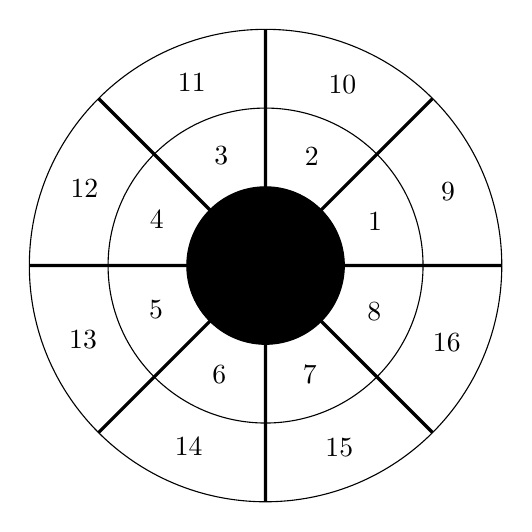
\begin{tikzpicture}
\draw [very thick] (-3,0) -- (3,0)
                   (-2.1213,-2.1213) -- (2.1213,2.1213)
                   (2.1213,-2.1213) -- (-2.1213,2.1213)
                   (0,-3) -- (0,3);
                   
\draw[black,fill=black] (0,0) circle[radius=1];
\edef\actioncounter{1}
\foreach \rad in {2,3} {
     \draw (0,0) circle[radius=\rad];
     
     \foreach [count=\i from 0,evaluate=\i as \y using int(\actioncounter)] \q in {22, 67, 112, 157, 202, 247, 292, 337} {
     	\pgfmathparse{\actioncounter+1};
     	\xdef\actioncounter{\pgfmathresult};
        \node at (\q:\rad-0.5) {\y};
     }
   }
\end{tikzpicture}

\label{fig:prey_actions} }
\subfigure[دامنه دید تعریف شده برای صیاد در محیط صید و صیاد]{
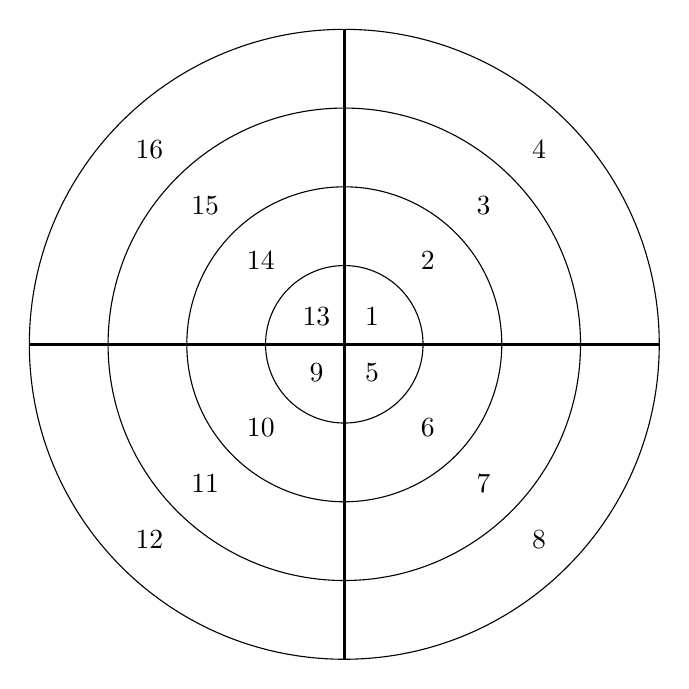
\begin{tikzpicture}
\draw [very thick] (-4,0) -- (4,0)
                   (0,-4) -- (0,4);
\foreach \rad in {1,2,3,4} {
     \draw (0,0) circle[radius=\rad];
     \foreach [count=\i from 0,evaluate=\i as \y using int(\rad+\i*4)] \q in {45,315,225,135}
        \node at (\q:\rad-0.5) {\y};
   }
\end{tikzpicture}
\label{fig:prey_vision} }
\caption{دامنه‌ی دید و حالت تعریف شده برای عامل صیاد در محیط صید و صیاد\مرجع{mohammad2015speedup}.}
\label{fig:prey_actions_vision}
\end{figure}
